\documentclass[9pt]{article}

\usepackage[margin=2cm]{geometry}
\usepackage{hyperref}
\usepackage{algorithm}
\usepackage{algpseudocode}
\usepackage{amsmath, amsthm, amssymb}
\usepackage{multicol}
\usepackage{tikz}
\usetikzlibrary{graphs}

\newtheorem{theorem}{Theorem}
\newtheorem{claim}{Claim}
\newtheorem{corollary}{Corollary}

\title{
    \textbf{CSE319: Modern Algorithm Design} \\
    \textbf{\large{Homework 2 Solutions}}
}
\author{
    \textbf{Submitted By:} \href{mailto:divyajeet21529@iiitd.ac.in}{Divyajeet Singh (2021529)}
    \hfill
    \textbf{Discussion Partner:} \href{mailto:siddhant21565@iiitd.ac.in}{Siddhant Rai Viksit (2021565)}
}
\date{}

\begin{document}
\maketitle

\section*{Solution 1.}
\subsection*{Part (a)}
In the naïve implementation, we regrow the tree (taking $O(m)$ time) after each price update.
We do this for each of the $O(n)$ iterations in one phase. We modify the BFS procedure to
ensure that the total work done in creating the search tree over $O(n)$ iterations of the
phase is $O(m)$. Along with a BFS-queue $Q$, we also maintain a set $S$ of currently
`\textit{un-tight}' edges, i.e.
\begin{equation}
    S = \{ (u, v) \in E \mid w(u, v) - p_{u} - p_{v} \neq 0, u \in Q \}
\end{equation}
\begin{figure}[htbp]
    \centering
    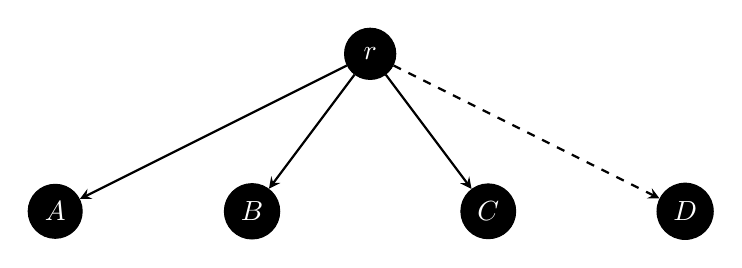
\begin{tikzpicture}[node distance=2cm, auto]
        \tikzstyle{node} = [draw, circle, minimum size=0.65cm, fill=black, text=white]
        \tikzstyle{tight} = [-{stealth}, thick]
        \tikzstyle{untight} = [-{stealth}, dashed, thick]
        \node[node] (R) at (0,0) {$r$};
        \node[node] (A) at (-4,-2) {$A$};
        \node[node] (B) at (-1.5,-2) {$B$};
        \node[node] (C) at (1.5,-2) {$C$};
        \node[node] (D) at (4,-2) {$D$};
        \path[tight]
        (R) edge node {} (A)
        (R) edge node {} (B)
        (R) edge node {} (C);
        \path[untight]
        (R) edge node {} (D);
    \end{tikzpicture}
    \caption{$(r, A)$, $(r, B)$, and $(r, C)$ are tight and added to $Q$. $(r, D)$ is un-tight and added to $S$.}
\end{figure}
\vspace*{0pt} \\
The idea is as follows. At the start of the phase, add $r \in L$ to $Q$. While $Q$ is not empty,
\begin{itemize}
    \item Pop a node $u$ from $Q$.
    \item For each edge $(u, v) \in E$, if $w(u, v) - p_{u} - p_{v} = 0$, add $v$ to $Q$,
    otherwise, add $(u, v)$ to $S$.
\end{itemize}
Once we get `\textit{stuck}', we perform a price update as usual for all explored vertices
in $L$ and $R$. Next, we find the edges in $S$ made tight by the price update\footnote{Note
that there can be multiple.}. Let these edges be
$T_{N} = \{ (u, v) \in S \mid w(u, v) - p_{u} - p_{v} = 0 \}$. We add the vertices
$V' = \{ v \mid (u, v) \in T_{N} \}$ to $Q$ and continue the BFS (as opposed to starting a
BFS from scratch). We repeat this process until a good path $P$ is found. \\
Since we grow one search tree per phase, each edge is considered at most twice (once while
adding it to $S$ and once while exploring it, if at all). Thus, the total work done searching
for good paths over all the $O(n)$ iterations of one phase is now $O(m)$. This obviously
excludes the work done to compute $\delta$s and update prices.

\subsection*{Part (b)}
We know that the value of $\delta$ for a price update can be computed in $O(m)$ per iteration
in each phase. For each phase, we also maintain a min-heap $H$, along with the BFS-queue $Q$
and set $S$. The heap is structured as $[\textsc{Priority}, \textsc{Item}]$.
\begin{equation}
    H = \{ [p_{v}, v] \mid (u, v) \in S \}
\end{equation}
Just like the set $S$, the heap $H$ is built incrementally. While BFS-ing, when we encounter
an un-tight edge $e = (u, v)$, we add $e$ to $S$ and $[p_{v}, v]$ to $H$. As expected, we
set\footnote{For consistency with $S$, we need to $\Call{Extract-min}{H}$ until $\Call{Top}{H}$
(the minimum value in $H$) exceeds the first selected $\delta$.}
\begin{equation}
    [\delta, \_] \gets \Call{Extract-min}{H}
\end{equation}
The time complexity of each extraction depends on the total number of elements $k$ in the heap.
There can be at most $n^{2}$ (non-distinct) elements in the heap during the phase. We do not
need to worry about duplicates since the extraction time is proportional to $\log{k}$, and
$\log{n^{2}} = 2 \log{n} = O(\log{n})$. Finally, there can be at most $O(m)$ inserts during the
search tree expansion and at most $O(m)$ extractions\footnote{$O(n)$ extractions should be
enough, but to take care of duplicates, we might need to extract all the elements inserted in
$H$.} overall during the phase. \\
Thus, the total time spent in computing $\delta$s over the entire phase is $O(m \log{n})$. This
yields an $O(mn \log{n})$ Hungarian Algorithm, as there can be at most $O(n)$ phases, and each
phase can be implemented in $O(m + m\log{n})$ time.

\section*{Solution 2.}
\subsection*{Part (a)}
We want to design a $\textsc{Poly}(n, k)$ algorithm to optimally solve the $k$-point facility
problem optimally on an edge-weighted path (line graph) of $n$ vertices. We do this with a
3-dimensional dynamic programming approach.

\subsubsection*{Dynamic Programming States}
Let $\Phi[i, v, \kappa]$ be the minimum cost of placing a total of $\kappa$ facilities
on the first $i$ vertices such that the last facility is placed at the vertex $v$. Then,
the optimal cost of placing $k$ facilities on the line graph is
$\min_{k \leq v \leq n} \Phi[n, v, k]$.

\subsubsection*{Base Cases}
Equation \ref{eq:base-case} describes the base cases.
\begin{equation}
    \label{eq:base-case}
    \Phi[i, v, \kappa] = \begin{cases}
        \infty & v > i \textbf{ or } \kappa > v \\
        \sum_{u = 1}^{i} d_{G}(u, v) & \kappa = 1 \\
    \end{cases}
\end{equation}
\begin{itemize}
    \item The first case covers the situations where the last facility is placed at a vertex
    $v$ after the first $i$ vertices, or when the number of facilities $\kappa$ is higher
    than the vertex $v$ at which the last facility is placed.
    \item The second case covers the actual base case. We place $\kappa = 1$ facilities at a
    vertex $v$. The cost of this placement is the sum of the distances of the first $i$
    vertices from the vertex $v$.
\end{itemize}

\subsubsection*{Recurrence Relation}
Equation \ref{eq:recurrence} describes the recurrence relation.
\begin{equation}
    \label{eq:recurrence}
    \Phi[i, v, \kappa] = \begin{cases}
        \Phi[i-1, v, \kappa] + d_{G}(v, i) & v < i \\
        \min_{1 \leq u < i} \left\{ \Phi[m-1, u, \kappa-1] + \sum_{w = m}^{i} d_{G}(w, i) \right\}
            & \text{otherwise}
    \end{cases}
\end{equation}
where, in the second case, $m$ is the leftmost vertex that is closer to $i$ than $u$.
\begin{itemize}
    \item The first case covers the situation when we do not place a facility at the current
    vertex $i$. This costs the same as placing $\kappa$ facilities on the first $i-1$ vertices
    with the last facility at $v$, and the distance between $i$ and its closest facility at $v$.
    \item The second case covers the situation when we place a facility at the current vertex
    $i$. This arrangement costs placing $\kappa-1$ facilities in the first $m-1$ vertices with
    the last facility at some $1 \leq u < i$ and the distance between $i$ and all vertices beyond
    $m$, where $m$ is the leftmost vertex that is closer to $i$ than $u$. We take the minimum
    over $u$ to find the optimal placement.
\end{itemize}

\subsubsection*{The Algorithm}
Let the edge weights on the line graph be $W_{E} = \{ w_{1}, w_{2}, \ldots, w_{n-1} \}$ from
left to right, where $w_{i} = d_{G}(i, i+1)$ for $i \in [n-1]$. We calculate the prefix sum
array $P[1:n]$ such that
\begin{equation}
    P[i+1] = \sum_{j=1}^{i} w_{j} = \sum_{j=1}^{i} d_{G}(j, j+1) \quad \forall i \in [n-1]
\end{equation}
\vfill
\pagebreak
\hspace*{-19pt}
Using the prefix sum array $P$, we gain immediate access to the distance between any two
vertices
\begin{equation}
    d_{G}(u, v) = d_{G}(v, u) = P[v] - P[u] \quad \forall u < v \in [n]
\end{equation}
We also need to calculate $m$ for any given $(i, j)$ pair. As per our requirement,
$m = \textsc{Median}_{G}(i, j)$ suffices, which denotes the middle point between $i$ and
$j$ with respect to the edge weights\footnote{We can pre-compute this in an array
$M[i, j] = \textsc{Median}_{G}(i, j)$ in $O(n^{2})$ time (see \textbf{Appendix})}. \\
A recursive implementation of the algorithm is given in Algorithm \ref{algo:line-dp}. The final
solution is given in Algorithm \ref{algo:line-k-point-facility}.
\begin{algorithm}[H]
    \caption{Recursive DP for the $k$-point Facility Problem on an edge-weighted path}
    \label{algo:line-dp}
    \begin{algorithmic}[1]
        \Procedure{Dp}{$i, v, \kappa$}:
            \If{$(i, v, \kappa) \in \Phi$} \Comment{Value already computed}
                \State \Return $\Phi[i, v, \kappa]$
            \ElsIf{$v < i$} \Comment{Do not place any facility at $i$ (Recurrence Case 1)}
                \State $\Phi[i, v, \kappa] \gets \Call{Dp}{i-1, v, \kappa} + d_{G}(v, i)$
                \State \Return $\Phi[i, v, \kappa]$
            \Else \Comment{Place a facility at $i$ (Recurrence Case 2)}
                \State $\varphi \gets \infty$
                \State $m_{\textbf{prev}} \gets M[i-1, i]$
                \State $s \gets 0$
                \For{$u \gets i-1$ to $1$}
                    \State $m \gets M[u, i]$
                    \For{$j \gets m_{\textbf{prev}}$ to $m$}
                        \State $s \gets s + d_{G}(j, i)$
                    \EndFor
                    \State $\varphi \gets \min \left( \varphi, \Call{Dp}{m-1, u, \kappa-1} + s \right)$
                    \State $m_{\textbf{prev}} \gets m$
                \EndFor
                \State $\Phi[i, v, \kappa] \gets \varphi$
                \State \Return $\Phi[i, v, \kappa]$
            \EndIf
        \EndProcedure
    \end{algorithmic}
\end{algorithm}
\vspace*{-12pt}
\begin{algorithm}[H]
    \caption{Solve the $k$-point Facility Problem on an edge-weighted path}
    \label{algo:line-k-point-facility}
    \begin{algorithmic}[1]
        \Procedure{$k$-point-facility-line}{$G = (V, E), k$}:
            \State $P \gets \textsc{Prefix-Sum}(W_{E})$ \Comment{$W_{E}$ can be obtained by a modified BFS}
            \State $M \gets \textsc{Pairwise-medians}(G)$
            \State $\Phi \gets \{ \}$ \Comment{An empty memoization table, indexed $[i, v, \kappa]$}
            \For{$v \gets 1$ to $n$}
                \State $s \gets 0$
                \For{$i \gets 1$ to $n$}
                    \State $s \gets s + d_{G}(v, i)$
                    \For{$\kappa \gets 1$ to $k$}
                        \If{$v > i$ \textbf{or} $\kappa > v$}
                            \State $\Phi[i, v, \kappa] \gets \infty$ \Comment{(Invalid) Base Case}
                        \EndIf
                    \EndFor
                    \State $\Phi[i, v, 1] \gets s$ \Comment{(Valid) Base Case}
                \EndFor
            \EndFor
            \State $\textsc{Opt} \gets \infty$
            \For{$v \gets k$ to $n$}
                \State $\textsc{Opt} \gets \min \left( \textsc{Opt}, \Call{Dp}{n, v, k} \right)$
            \EndFor
            \State \Return $\textsc{Opt}$
        \EndProcedure
    \end{algorithmic}
\end{algorithm}
\vfill
\pagebreak
\hspace*{-19pt}
In Algorithm \ref{algo:line-k-point-facility}, we initalize the the base cases of the DP table
$\Phi$ in $O(n^{2} k)$ time. By iterating over $v$ in the outer loop, we can calculate a running
sum to avoid recomputing the distances between $i$ and $v$ for each $i$. \\
Algorithm \ref{algo:line-dp} has been written with a slightly non-trivial optimization. In
Recurrence Case 2, one might want to compute the sum $\sum_{j=m}^{i} d_{G}(j, i)$ naïvely for
as per \ref{eq:recurrence}, resulting in an effort of $O(n)$ for each $u$. Instead, we loop
over $u$ in reverse and maintain a running sum of the distances between $j$ and $i$ for each
$j$ from $m_{\textbf{prev}}$ to $m$. This saves duplicate calculations, as $m$ decreases
monotonically as $u$ decreases - an overall total effort of $O(n)$.

\subsubsection*{Backtracking to find the set $C$}
To find the actual set $C \subseteq V$, we need to backtrack through the table $\Phi[i, v, \kappa]$.
We start at $\Phi[i=n, v=n, \kappa=k]$, and decrease $v$ until we find the first
$\Phi[i, v, \kappa] \neq \Phi[i, v-1, \kappa]$, and add this $v$ to $C$. We then repeat this
process from $\Phi[v-1, v-1, k-1]$ until we have $k$ vertices in $C$. Again, the exact algorithm
is given in the \textbf{Appendix}.

\subsubsection*{Time Complexity}
There are a total of $O(n^{2} k)$ subproblems. Given the preprocessing and optimizations, we
see that
\begin{itemize}
    \item We spend an $O(n^{2} k)$ effort to initialize the base cases.
    \item A total of $n$ states, where $i = v$, are computed in $O(n)$ time, adding another
    $O(n^{2})$ effort.
    \item The rest of the states are computed in constant time, thanks to memoization.
    \item $O(n + k)$ time is spent backtracking to find the set $C$, if required.
\end{itemize}
Thus, the overall time complexity of the solution is $O(n^{2} k) = \textsc{Poly}(n, k)$.
We could have still achieved a $\textsc{Poly}(n, k)$ runtime by removing the
optimization tricks (resulting in a $O(n^{3} k)$ complexity), but \textit{efficieny} :)

\subsection*{Part (b)}
We are given an algorithm $\mathcal{A}$ that solves the $k$-point facility problem optimally
on trees. We need to show that an algorithm that samples a tree $T$ from an $\alpha$-stretch
distribution and runs $\mathcal{A}$ on $T$ to get $C_{T}$ ensures
\begin{equation}
    \mathbb{E}_{T}[\Phi_{T}(C_{T})] \leq \alpha \cdot \textsc{Opt}
\end{equation}
Note that we calculate $\Phi_{T}(C_{T})$ as opposed to $\Phi_{G}(C_{T})$, since we solve the
$k$-point facility problem on the tree $T$. We simply expand $\Phi_{T}(C_{T})$ and use
linearity of expectation.
\begin{align}
    \begin{split}
        \mathbb{E}_{T}[\Phi_{T}(C_{T})] &= \mathbb{E}_{T} \left[ \sum_{v \in V} d_{T}(v, C_{T}) \right] \\
        &= \sum_{v \in V} \mathbb{E}_{T} \left[ \min_{c \in C_{T}} d_{T}(v, c) \right] \\
        &= \sum_{v \in V} \mathbb{E}_{T} \left[ d_{T}(v, c^{*}_{v}) \right]
        \qquad \text{where } c^{*}_{v} = \underset{c \in C_{T}}{\text{argmin}} \ d_{T}(v, c) \\
        &\leq \sum_{v \in V} \alpha \cdot d_{G}(v, c^{*}_{v})
        = \alpha \cdot \textsc{Opt}
    \end{split}
\end{align}
where the inequality holds due to the $\alpha$-stretch property of the distribution.

\subsection*{Part (c)}
Now, we perform $L = O \left( \frac{\log{n}}{\epsilon} \right)$ independent runs of the above
algorithm, to get the sets $C_{1}, C_{2}, \ldots, C_{L}$ from the trees
$T_{1}, T_{2}, \ldots, T_{L}$ sampled from the $\alpha$-stretch distribution. We want to
bound the probability that $\Phi_{T^{*}}(C^{*})$ exceeds the expected cost by a factor of
$1 + \epsilon$, where $T^{*}$ is the tree that gives the set
$C^{*} = \underset{i \in [L]}{\text{argmin}} \ \Phi_{T_{i}}(C_{i})$. \\
We first find the probability that for any tree $T_{i}$,
\begin{align}
    \begin{split}
        \mathbb{P}[\Phi_{T_{i}}(C_{i}) \geq (1 + \epsilon) \cdot \alpha \cdot \textsc{Opt}]
        &\leq \frac{\mathbb{E}_{T_{i}}[\Phi_{T_{i}}(C_{i})]}{(1 + \epsilon) \cdot \alpha \cdot \textsc{Opt}}
        \qquad \text{by Markov's Inequality} \\
        &\leq \frac{1}{1 + \epsilon} \qquad \text{by the $\alpha$-stretch property}
    \end{split}
\end{align}
Now, the probability that the cost of the minimizing tree-set $C^{*}$ exceeds some value is the
probability that the cost of all tree-sets exceeds that value. So, we have
\begin{align}
    \begin{split}
        \mathbb{P}[\Phi_{T^{*}}(C^{*}) \geq (1 + \epsilon) \cdot \alpha \cdot \textsc{Opt}]
        &\leq \mathbb{P} \left[ \bigcap_{i=1}^{L} \{ \Phi_{T_{i}}(C_{i}) \geq (1 + \epsilon) \cdot \alpha \cdot \textsc{Opt} \} \right] \\
        &= \prod_{i=1}^{L} \mathbb{P}[\Phi_{T_{i}}(C_{i}) \geq (1 + \epsilon) \cdot \alpha \cdot \textsc{Opt}]
        \qquad \text{by independence} \\
        &\leq \left( \frac{1}{1 + \epsilon} \right)^{L}
    \end{split}
\end{align}
Let $L = c \cdot \frac{\log{n}}{\epsilon}$ for some constant $c \in \mathbb{R}_{\geq 0}$.
Then, we have
\begin{align}
    \begin{split}
        \mathbb{P}[\Phi_{T^{*}}(C^{*}) \geq (1 + \epsilon) \cdot \alpha \cdot \textsc{Opt}]
        &\leq \left( \frac{1}{1 + \epsilon} \right)^{c \cdot \frac{\log{n}}{\epsilon}} \\
        &= \left( 1 + \epsilon \right)^{-c \cdot \frac{\log{n}}{\epsilon}} \\
        &\leq \left( e^{\epsilon} \right)^{-c \cdot \frac{\log{n}}{\epsilon}} \quad \text{since }
        1 + x \leq e^{x} \ \forall x \in \mathbb{R} \\
        &= \frac{1}{e^{c \log{n}}} = \frac{1}{n^{k}} = \frac{1}{\textsc{Poly}(n)}
    \end{split}
\end{align}
where $k$ absorbs the logarithmic conversion factor.

\subsection*{Part (d)}
We want to show that the expected weight of a low-stretch tree with expected stretch $\alpha$
is at most $O(\alpha)$ times the weight of a minimum spanning tree, i.e.,
\begin{equation}
    \mathbb{E}_{\textsc{Lst}}[w(\textsc{Lst})] \leq O(\alpha) \cdot w(\textsc{Mst})
\end{equation}
\begin{claim}
    \label{claim:tree-equality}
    Let $T_{1}$ and $T_{2}$ be any two spanning trees of a graph $G$. Then,
    \begin{equation}
        \bigcup_{(u, v) \in T_{1}} P_{T_{2}}(u, v) = T_{2}
    \end{equation}
    where $P_{T}(x, y) = (v_{1} \to v_{2} \to \cdots \to v_{k})$ denotes the path from $x$ to
    $y$ in a spanning tree $T$, with $v_{1} = x$ and $v_{k} = y$.
\end{claim}
\begin{quote}
\textit{Proof.}
    Suppose $T_{2}$ is rooted at some $r \in T_{2}$. Then, every edge
    $\textsc{Par}_{T_{2}}(y) = (x, y)$ can be said to be the parent of the vertex $y$ in
    $T_{2}$. Let the sub-tree of $T_{2}$ rooted at $v \in T_{2}$ be $\textsc{Sub}_{T_{2}}(v)$.
    Then, for any $(u, v) \in T_{1}$, we have either of the two cases
    \begin{enumerate}
        \item $v \in T_{2} \setminus \textsc{Sub}_{T_{2}}(u)$, i.e. $v$ is not in the sub-tree
        of $u$ in $T_{2}$. Then, $\textsc{Par}_{T_{2}}(u) \in P_{T_{2}}(u, v)$.
        \item $v \notin T_{2} \setminus \textsc{Sub}_{T_{2}}(u)$, i.e. $v$ is in the sub-tree
        of $u$ in $T_{2}$. $v$ is connected to all other vertices in this sub-tree. Then, there
        must be some $x \in \textsc{Sub}_{T_{2}}(u)$ and
        $y \in T_{2} \setminus \textsc{Sub}_{T_{2}}(u)$, such that $(x, y) \in T_{1}$, otherwise
        $T_{1}$ would not be spanning. So, we have an edge $(x, y) \in T_{1}$ such that
        $y \in T_{2} \setminus \textsc{Sub}_{T_{2}}(x)$, and thus, by case 1,
        $\textsc{Par}_{T_{2}}(u) \in P_{T_{2}}(x, y)$.
    \end{enumerate}
This means that each edge (`\textit{parent}' of some vertex) in $T_{2}$ is covered by at least
some edge in $T_{1}$.
\hfill $\square$
\end{quote}
Claim \ref{claim:tree-equality} holds for any two general spanning trees. Now consider an
\textsc{Lst} and an \textsc{Mst} of the graph $G$. We have by the $\alpha$-stretch property
of the \textsc{Lst} that
\begin{align}
    \label{eq:MST-LST}
    \begin{split}
        \mathbb{E}_{\textsc{Lst}}[d_{\textsc{Lst}}(x, y)] &\leq \alpha \cdot d_{G}(x, y) \qquad \forall \ x, y \in V \\
        \implies \sum_{(x, y) \in \textsc{Mst}} \mathbb{E}_{\textsc{Lst}}[d_{\textsc{Lst}}(x, y)] &\leq \sum_{(x, y) \in \textsc{Mst}} \alpha \cdot d_{G}(x, y) \\
        \implies \sum_{(x, y) \in \textsc{Mst}} \sum_{(u, v) \in P_{\textsc{Lst}}(x, y)} \mathbb{E}_{\textsc{Lst}}[d_{\textsc{Lst}}(u, v)] &\leq \alpha \cdot w(\textsc{Mst})
    \end{split}
\end{align}
By Claim \ref{claim:tree-equality} we have (where $T_{1} = \textsc{Mst}$ and
$T_{2} = \textsc{Lst}$)
\begin{align}
    \label{eq:MST-LST-claim}
    \begin{split}
        \bigcup_{(x, y) \in \textsc{Mst}} P_{\textsc{Lst}}(x, y) &= \textsc{Lst} \\
        \mathbb{E}_{\textsc{Lst}}[w(\textsc{Lst})] = \mathbb{E}_{\textsc{Lst}}\left[ w \left( \bigcup_{(x, y) \in \textsc{Mst}} P_{\textsc{Lst}}(x, y) \right) \right]
        &\leq \sum_{(x, y) \in \textsc{Mst}} \mathbb{E}_{\textsc{Lst}}[ w(P_{\textsc{Lst}}(x, y))] \\
        &= \sum_{(x, y) \in \textsc{Mst}} \sum_{(u, v) \in P_{\textsc{Lst}}(x, y)} \mathbb{E}_{\textsc{Lst}}[d_{\textsc{Lst}}(u, v)]
    \end{split}
\end{align}
where the inequality follows due to the Union bound. By \ref{eq:MST-LST} and
\ref{eq:MST-LST-claim}, we get
\begin{equation}
    \mathbb{E}_{\textsc{Lst}}[w(\textsc{Lst})] \leq \alpha \cdot w(\textsc{Mst})
\end{equation}

\subsection*{Part (e)}

\section*{Solution 3.}
\subsection*{Part (a)}
We need to show that for all $x, y \in V$, even if $(x, y) \notin E$,
\begin{equation}
    d_{G}(x, y) \leq d_{H}(x, y) \leq \gamma \cdot d_{G}(x, y)
\end{equation}
The first inequality holds trivially, since the $\gamma$-distance emulator $H$ is a subgraph of
$G$, so, $d_{G}(x, y) \leq d_{H}(x, y)$. The second inequality also holds trivially for
$(x, y) \in E$ by the definition of $\gamma$-distance emulator. If $(x, y) \notin E$, then
consider the shortest path $P^{*}_{G}(x, y) = (v_{1} \to v_{2} \to \ldots \to v_{k})$ in $G$,
where $v_{1} = x$ and $v_{k} = y$, and each edge $(v_{i}, v_{i+1}) \in E$.
\begin{align}
    \begin{split}
        d_{G}(x, y) &= \sum_{i=1}^{k-1} d_{G}(v_{i}, v_{i+1}) \\
        &\geq \sum_{i=1}^{k-1} \frac{1}{\gamma} \cdot d_{H}(v_{i}, v_{i+1}) \\
        \implies \gamma \cdot d_{G}(x, y) &\geq \sum_{i=1}^{k-1} d_{H}(v_{i}, v_{i+1})
    \end{split}
\end{align}
Since $H \subseteq G$, some edges $P^{*}_{G}(x, y)$ may not be in $H$. So, $P^{*}_{G}(x, y)$
may not be the shortest $x$-$y$ path in $H$. This means that
\begin{align}
    d_{H}(x, y) &\leq \sum_{i=1}^{k-1} d_{H}(v_{i}, v_{i+1}) \leq \gamma \cdot d_{G}(x, y)
\end{align}

\subsection*{Part (b)}
By \textit{Construction 1.}, we have $t = 4 \log{n}$ trees, $T_{1}$, $T_{2}$, $\ldots$,
$T_{t}$, sampled from a randomized $\alpha$-stretch spanning tree distribution. We are given
that the distance emulator $H$ is the union of all these trees.

\subsubsection*{Subpart (i)}
For any fixed edge $(x, y) \in E$, we bound the probability that the shortest $x$-$y$ distance
in some fixed tree $T_{i}$ (i.e. a fixed $i$) is at least $2 \alpha \cdot d_{G}(x, y)$.
\begin{align}
    \begin{split}
        \mathbb{P}[d_{T_{i}}(x, y) \geq 2 \alpha \cdot d_{G}(x, y)]
        &\leq \frac{\mathbb{E}_{T_{i}}[d_{T_{i}}(x, y)]}{2 \alpha \cdot d_{G}(x, y)} \qquad \text{by Markov's Inequality} \\
        &\leq \frac{1}{2} \qquad \text{by the $\alpha$-stretch property}
    \end{split}
\end{align}
Now, since $H$ contains all the edges present in all the trees, the probability that the shortest
$x$-$y$ distance in $H$ is at least $2 \alpha \cdot d_{G}(x, y)$ is the probability that the
shortest $x$-$y$ distance in all the trees is at least $2 \alpha \cdot d_{G}(x, y)$. So,
\begin{align}
    \begin{split}
        \mathbb{P}[d_{H}(x, y) \geq 2 \alpha \cdot d_{G}(x, y)]
        &\leq \mathbb{P} \left[ \bigcap_{i=1}^{t} \{ d_{T_{i}}(x, y) \geq 2 \alpha \cdot d_{G}(x, y) \} \right] \\
        &= \prod_{i=1}^{t} \mathbb{P}[d_{T_{i}}(x, y) \geq 2 \alpha \cdot d_{G}(x, y)] \qquad \text{by independence} \\
        &\leq \left( \frac{1}{2} \right)^{t} = 2^{-t} = \frac{1}{n^{4}}
    \end{split}
\end{align}

\subsubsection*{Subpart (ii)}
We know that there always exists a low-stretch spanning tree distribution with a stretch of
$\alpha = O(\log{n} \log{\log{n}})$ for any graph $G$ with $n$ vertices\footnote{\textbf{Mistake
in question:} Lecture notes suggest a stretch of $O(\log{n} \log{\log{n}})$ for general graphs
instead of $O(n \log{n} \log{\log{n}})$.}. So, let the stretch for a graph $G = (V, E)$ be
$\alpha = c \log{n} \log{\log{n}}$ for some constant $c \in \mathbb{R}_{\geq 0}$. Then, we have
\begin{equation}
    \mathbb{P}[d_{H}(x, y) \geq 2 \cdot c \log{n} \log{\log{n}} \cdot d_{G}(x, y)] \leq \frac{1}{n^{4}}
\end{equation}
for a fixed edge $(x, y) \in E$. Now, we find the probability that no edge in $E$ has a stretch
greater than $2 \alpha$.
\begin{align}
    \begin{split}
        \mathbb{P}[\forall \ (x, y) \in E, d_{H}(x, y) \leq 2 \alpha \cdot d_{G}(x, y)]
        &= \mathbb{P} \left[ \bigcap_{(x, y) \in E} \{ d_{H}(x, y) \leq 2 \alpha \cdot d_{G}(x, y) \} \right] \\
        &= 1 - \mathbb{P} \left[ \bigcup_{(x, y) \in E} \{ d_{H}(x, y) \geq 2 \alpha \cdot d_{G}(x, y) \} \right] \\
        &\geq 1 - \sum_{(x, y) \in E} \mathbb{P}[d_{H}(x, y) \geq 2 \alpha \cdot d_{G}(x, y)] \qquad \text{by Union Bound} \\
        &\geq 1 - |E| \cdot \frac{1}{n^{4}} \geq 1 - \frac{n^{2}}{n^{4}} = 1 - \frac{1}{n^{2}}
    \end{split}
\end{align}
So, with probability at least $1 - \frac{1}{n^{2}}$, no edge in $G$ has a stretch greater than
$2 c \log{n} \log{\log{n}}$. But that means $H$ is a $(2c \log{n} \log{\log{n}})$-distance emulator
for $G$ with probability at least $1 - \frac{1}{n^{2}}$. Moreover, the number of edges in $H$
can be bounded by
\begin{equation}
    \lvert E_{H} \rvert = \left\lvert \bigcup_{i=1}^{t} E_{T_{i}} \right\rvert
    \leq \sum_{i=1}^{t} \lvert E_{T_{i}} \rvert
    = t \cdot (n-1) = 4 \log{n} \cdot (n-1) = O(n \log{n})
\end{equation}
Thus, $H$ is an $O(n \log{n})$-sized $O(\log{n} \log{\log{n}})$-distance emulator for $G$ with
probability at least $1 - \frac{1}{n^{2}}$.

\subsection*{Part (c)}
\subsubsection*{Subpart (i)}
We are given a graph $G$ with girth strictly greater than $g$. We work towards \textbf{Sub-subpart (C)}.
\vspace*{10pt} \\
\textbf{Sub-subpart (A)}
\vspace*{5pt} \\
Given that the average degree of the graph $G$ is $\bar{d} = \frac{2m}{n}$. We show how to
construct a feasible subset $S \subseteq V$ such that the induced subgraph $H := G[S]$ has minimum
degree at least $\frac{\bar{d}}{2}$. Algorithm \ref{alg:subpart-c} describes the construction of
such a subset $S$.
\begin{algorithm}
    \caption{Constructing a feasible set $S \subseteq V$}
    \label{alg:subpart-c}
    \begin{algorithmic}[1]
        \Procedure{Construct-feasible-set}{$G = (V, E)$}:
            \State $S \gets V$
            \While{$\exists \ v \in S$ with $d_{H}(v) < \frac{\bar{d}}{2}$}
                \State $S \gets S \setminus \{v\}$
            \EndWhile
            \State \Return $S$
        \EndProcedure
    \end{algorithmic}
\end{algorithm}
\vspace*{0pt} \\
We only need to show that the algorithm terminates without emptying $S$ completely. The removal
of a vertex $v \in S$ with $d_{G}(v) < \frac{\bar{d}}{2}$, the number of edges goes down by at
most $\frac{\bar{d}}{2} - 1 = \frac{m}{n} - 1$. Let us assume, for the sake of contradiction,
that at the end of the algorithm, $S = \emptyset$. Then, the total number of edges removed would
be at most
\begin{equation}
    \sum_{v \in V} \frac{m}{n} - 1 = m - n < m
\end{equation}
This means that we have deleted all vertices, but some edges still remain in $G[S]$, which is
absurd. Thus, an $S$ produced by Algorithm \ref{alg:subpart-c} is feasible, and therefore such
an $S$ exists.
\vspace*{10pt} \\
\textbf{Sub-subpart (B)}
\vspace*{5pt} \\
In such a subgraph $H$, we show that for any $v \in H$,
\begin{equation}
    \left\lvert \textsc{Bfs}\left(H, v, \frac{g}{2} \right) \right\rvert
    \geq \left( \frac{\bar{d}}{2} - 1 \right)^{\left\lfloor \frac{g}{2} \right\rvert}
\end{equation}
where the girth of the graph is strictly greater than some $g$, and $\textsc{Bfs}(G, v, k)$
denotes the set of vertices reacheable from $v$ in at most $k$ steps in the graph $G$. \\
This is now an easy job. We know that the minimum degree of any vertex in $H$ is $\frac{\bar{d}}{2}$.
So, in the first hop from a vertex $v$, we can reach at least $\frac{\bar{d}}{2}$ new vertices.
In the  second hop, we discover at least $\frac{\bar{d}}{2} - 1$ vertices from each of the
$\frac{\bar{d}}{2}$ vertices discovered in the first step. In each subsequent hop $i$, we
encounter at least $n_{i-1} \cdot \left( \frac{\bar{d}}{2} - 1 \right)$ new vertices, where
$n_{i-1}$ is the number of vertices discovered in the $(i-1)^{th}$ hop, and the $-1$ accounts
for the vertex we came from. So, we have the total number of distinct vertices as
\begin{align}
    \begin{split}
        \left\lvert \textsc{Bfs}\left(H, v, \frac{g}{2} \right) \right\rvert
        &= \frac{\bar{d}}{2} + \frac{\bar{d}}{2} \cdot \left( \frac{\bar{d}}{2} - 1 \right)
        + \frac{\bar{d}}{2} \cdot \left( \frac{\bar{d}}{2} - 1 \right)^{2} + \cdots
        + \frac{\bar{d}}{2} \cdot \left( \frac{\bar{d}}{2} - 1 \right)^{\left\lfloor \frac{g}{2} \right\rfloor - 1} \\
        &= \frac{\bar{d}}{2} \cdot \frac{\left( \frac{\bar{d}}{2} - 1 \right)^{\left\lfloor \frac{g}{2} \right\rfloor} - 1}{\frac{\bar{d}}{2} - 2} \\
        &\geq \left( \frac{\bar{d}}{2} - 1 \right)^{\left\lfloor \frac{g}{2} \right\rfloor}
        \qquad \text{since } \frac{x}{x - 2} \geq 1 \ \forall \ x \geq 2
    \end{split}
\end{align}
We can rest assured that the counted vertices are distinct by crucially using the fact that
the girth of the graph is strictly greater than $g$, but the hops in all directions can
achieve a maximum spread of $2 \cdot \left\lfloor \frac{g}{2} \right\rfloor \leq g$.
\vspace*{10pt} \\
\textbf{Sub-subpart (C)}
\vspace*{5pt} \\
At this point, we have a set $S$ such that the induced subgraph $H := G[S]$ has minimum degree
at least $\frac{\bar{d}}{2}$, and we have seen that the BFS-tree from any vertex $v \in H$ has
at least $\left( \frac{\bar{d}}{2} - 1 \right)^{\left\lfloor \frac{g}{2} \right\rfloor}$ vertices.
Clearly, a BFS-tree of depth $\left\lfloor \frac{g}{2} \right\rfloor$ from any vertex $v \in H$
contains at most the total number of vertices in $G$. So, we have
\begin{align}
    \begin{split}
        \left( \frac{\bar{d}}{2} - 1 \right)^{\left\lfloor \frac{g}{2} \right\rfloor} &\leq n \\
        \implies \frac{\bar{d}}{2} &\leq 1 + n^{\frac{1}{\left\lfloor \frac{g}{2} \right\rfloor}} \\
    \end{split}
\end{align}
Note that since $\bar{d} = \frac{2m}{n}$, we can write\footnote{Technically,
$O \left( n + n^{1 + \frac{1}{\left\lfloor \frac{g}{2} \right\rfloor}} \right)
= O \left( n^{1 + \frac{1}{\left\lfloor \frac{g}{2} \right\rfloor}} \right)$.}
\begin{equation}
    m = \frac{n \bar{d}}{2} \leq n \cdot \left( 1 + n^{\frac{1}{\left\lfloor \frac{g}{2} \right\rfloor}} \right)
    = n + n^{1 + \frac{1}{\left\lfloor \frac{g}{2} \right\rfloor}}
    = O \left( n + n^{1 + \frac{1}{\left\lfloor \frac{g}{2} \right\rfloor}} \right)
\end{equation}

\subsubsection*{Subpart (ii)}
We are given a variant of Kruskal's algorithm for $\alpha \geq 1$. We start with an empty $H$
and add each edge $(x, y) \in E$ to $H$ if $d_{H}(x, y) > \alpha \cdot d_{G}(x, y)$.
\vspace*{10pt} \\
\textbf{Sub-subpart (A)}
\vspace*{5pt} \\
We first show that at $\alpha = n - 1$, the described procedure becomes Kruskal's algorithm.
We note that an edge $e_{i} = (x, y) \in E$ is included in $H_{i}$ if
\begin{equation}
    d_{H_{i-1}}(x, y) > (n - 1) \cdot d_{G}(x, y)
\end{equation}
Let us analyze what happens when the algorithm encounters an edge $e_{i} = (x, y) \in E$.
We land in one of two scenarios:
\begin{enumerate}
    \item $x$ and $y$ are in different connected components of $H_{i-1}$. Then,
    \begin{equation}
        d_{H_{i-1}}(x, y) = \infty > (n - 1) \cdot d_{G}(x, y)
    \end{equation}
    satisfying the required condition. So, $H_{i} \gets H_{i-1} \cup \{ e_{i} \}$, i.e. $x$ and
    $y$ get connected in $H_{i}$. Note that when an edge gets added in the $i^{th}$ iteration,
    $d_{H_{j}}(x, y) \leq (n - 1) \cdot d_{G}(x, y)$ for all $j \geq i$.
    \item $x$ and $y$ are in the same connected component of $H_{i-1}$. By defintion of a connected
    component, there exists a path $P_{H_{i-1}}(x, y) = (v_{1} \to v_{2} \to \ldots \to v_{k})$
    in $H_{i-1}$, where $v_{1} = x$ and $v_{k} = y$, and each edge $(v_{j}, v_{j+1}) \in H_{i-1}$.
    \begin{align}
        \begin{split}
            d_{H_{i-1}}(x, y) &= \sum_{j=1}^{k-1} d_{H_{i-1}}(v_{j}, v_{j+1}) \\
            &= \sum_{j=1}^{k-1} d_{G}(v_{j}, v_{j+1}) \\
            &\leq k \cdot w^{*} \qquad \text{where } w^{*} = \max_{j \in [k-1]} d_{G}(v_{j}, v_{j+1}) \\
            &\leq (n - 1) \cdot d_{G}(x, y)
        \end{split}
    \end{align}
    where the last inequality holds because
    \begin{itemize}
        \item There can be at most $n - 1$ edges in the path $P_{H_{i-1}}(x, y)$.
        \item $w^{*} = w_{e_{i}} = d_{G}(x, y)$, since $e_{i}$ must be the heaviest edge
        considered so far.
    \end{itemize}
    This does not satisfy the required condition. So, $H_{i} \gets H_{i-1}$.
\end{enumerate}
The above two points combined show that an edge $e_{i} = (x, y) \in E$ is included in $H_{i}$
if $x$ and $y$ are in different connected components of $H_{i-1}$. This is exactly the behavior
of Kruskal's algorithm, as adding the exact edges that are in different connected components
each time ensures that no cycles are formed. \\
By the equivalence thus proved, $H$ is not only a subgraph, but also a spanning tree. The
procedure ensures that $d_{H_{|E|}}(x, y) \leq (n - 1) \cdot d_{G}(x, y)$ for each edge
$(x, y) \in E$, thus making $H$ an $(n-1)$-distance emulator. Moreover, since we showed in
\textbf{Problem 3 (a)} that even if $(x, y) \notin E$,
$d_{H_{|E|}}(x, y) \leq (n - 1) \cdot d_{G}(x, y)$ by the distance emulator property, $H$ is
an $(n-1)$-stretch spanning tree of $G$.
\vspace*{10pt} \\
\textbf{Sub-subpart (B)}
\vspace*{5pt} \\
Finally, we set $\alpha = O(\log{n})$ for a graph whose girth is strictly more than
$g = \Theta(\log{n})$. Given $g$, we know that
\begin{equation}
    m \leq c \cdot \left( n + n^{1 + \frac{1}{\left\lfloor \frac{\log{n}}{2} \right\rfloor}} \right)
    = c \cdot n \cdot \left( 1 + n^{\frac{2}{\log{n}}} \right)
    = c \cdot k \cdot n = O(n) \qquad \text{where } k \geq 5
\end{equation}
with the help of the following equation
\begin{align}
    \begin{split}
        \lim_{n \to \infty} 1 + n^{\frac{2}{\log{n}}}
        &= 1 + \lim_{n \to \infty} \left( 2^{\log{n}} \right)^{\frac{2}{\log{n}}} = 1 + 2^{2} = 5
    \end{split}
\end{align}
$H \subseteq G$ is an $O(\log{n})$-distance emulator, because one of two things can happen
when considering an edge $e_{i} = (x, y) \in E$:
\begin{enumerate}
    \item $d_{H_{i-1}}(x, y) \leq O(\log{n}) \cdot d_{G}(x, y)$. In this case, we leave
     $H_{i-1}$ unchanged, as the distance emulator property is satisfied for $e_{i}$.
    \item $d_{H_{i-1}}(x, y) > O(\log{n}) \cdot d_{G}(x, y)$. So, $e_{i}$ is added to
    $H_{i-1}$ to obtain $H_{i}$. Now,
    $d_{H_{i}}(x, y) = d_{G}(x, y) \leq O(\log{n}) \cdot d_{G}(x, y)$, i.e. the distance
    emulator property will now remain satisfied for $e_{i}$.
\end{enumerate}
Hence, $H$ is an $O(\log{n})$-distance emulator of $G$ with $O(n)$ edges.

\section*{Appendix}
\subsection*{Problem 2 (a)}
\subsubsection*{Finding the Prefix Sum Array}
The algorithm to find the prefix sum array of the array of weights $W[1:n-1]$, where
$W[i] = d_{G}(i, i+1)$, is given in Algorithm \ref{alg:prefix-sum}. We pay close attention
to the indices, as $|W| = n-1$ but $|P| = n$.
\begin{algorithm}
    \caption{Computing the prefix sum array}
    \label{alg:prefix-sum}
    \begin{algorithmic}[1]
        \Procedure{Prefix-sum}{$W[1:n-1]$}:
            \State $P[1:n] \gets 0$
            \State $P[2] \gets W[1]$
            \For{$i \gets 3$ to $n$}
                \State $P[i] \gets P[i-1] + W[i]$
            \EndFor
            \State \Return $P$
        \EndProcedure
    \end{algorithmic}
\end{algorithm}

\subsubsection*{Finding Medians for all Pairs of Vertices}
The median of the distances between all pairs of vertices $(u, v)$ for $u < v$ on the edge-weighted
line graph $G$ can be computed in $O(n^{2})$ time using Algorithm \ref{alg:line-graph-median}.
\begin{algorithm}
    \caption{Computing the median of all pairs of vertices}
    \label{alg:line-graph-median}
    \begin{algorithmic}[1]
        \Procedure{Pairwise-medians}{$G = (V, E)$}:
            \State $M[1:n, 1:n] \gets 0$
            \For{$i \gets 1$ to $n$} \Comment{$\textbf{for}_{\textbf{out}}$}
                \State $m \gets i$
                \For{$j \gets i+1$ to $n$} \Comment{$\textbf{for}_{\textbf{in}}$}
                    \While{$d_{G}(i, m) < d_{G}(m, j)$}
                        \State $m \gets m + 1$
                    \EndWhile
                    \State $M[i, j] \gets m$
                \EndFor
            \EndFor
            \State \Return $M$
        \EndProcedure
    \end{algorithmic}
\end{algorithm}
\vspace*{0pt} \\
Strictly speaking, $M[i, j]$ stores the first vertex $m$ which is closer to $j$ than to $i$,
which is what we require. $\textbf{for}_{\textbf{out}}$ runs for a total of $O(n)$
iterations. For each $i$, $m$ starts at $i$ and moves to the right. At the end of each
iteration of the $\textbf{for}_{\textbf{out}}$, $m$ can be at most $n$. This means that $m$
travels a distance of at most $O(n)$ over the $O(n)$ iterations of $\textbf{for}_{\textbf{in}}$
for each $i$. Therefore, for each $i$, the total work done is $O(n)$. Hence, the overall time
complexity of the algorithm is $O(n^{2})$.

\subsubsection*{Backtracking  to find the set $C$}
Algorithm \ref{algo:backtrack} describes the backtracking procedure to find the set $C$,
assuming the dynamic programming table $\Phi[i, v, \kappa]$ is ready.
\begin{algorithm}[H]
    \caption{Backtrack to find the set $C$}
    \label{algo:backtrack}
    \begin{algorithmic}[1]
        \Procedure{Backtrack}{$\Phi[1:n, 1:n, 1:k]$}:
            \State $C \gets \{ \}$
            \State $i, v, \kappa \gets n, n, k$
            \While{$|C| \neq k$}
                \While{$\Phi[i, v, \kappa] = \Phi[i, v - 1, \kappa]$}
                    \State $v \gets v - 1$
                \EndWhile
                \State $C \gets C \cup \{ v \}$
                \State $i, v, \kappa \gets v-1, v-1, \kappa-1$
            \EndWhile
            \State \Return $C$
        \EndProcedure
    \end{algorithmic}
\end{algorithm}
\hspace*{-19pt}
The procedure takes only $O(n + k)$ time to find the set $C$. This is because we do not visit
all states $[i, v, \kappa]$ in the table. Instead, we visit at most $n$ states, where some
states are visited for $\kappa = 1$, some for $\kappa = 2$, and so on. Over the $k$
iterations of the outer $\textbf{while}$ loop, we visit $n$ states. \\
Informally, we can imagine it like a 3-dimensional staircase, where we start from the bottom
and climb up when we find a vertex to add to $C$. We can only move up exactly $k$ times, but
we might have to move left and back at most $n$ times.

\end{document}